\section{Zielsetzung}
\label{sec:ziel}

Ziel des Versuches ist es grundlegende Eigenschaften von Licht herauszufinden. Es werden hierfür
Elektronen mithilfe monochromatischen Lichtes aus einer Metalloberfläche gelöst.
Um dieses Phönomen erklären zu können, ist nur die Quantenelektrodynamik fähig und es ist deshalb notwendig sich mit dieser
näher zu beschäftigen.

\section{Theorie}
\label{sec:Theorie}

Um das Herauslösen der Elektronen aus der geladenen Metalloberfläche, also den Photoeffekt, verstehen zu können, wird die Korpuskeltheorie von Einstein verwendet.
Da es nicht möglich ist mithilfe der Maxwell'schen Gleichungen und dem daraus folgenden Wellencharakter des Lichtes diesen Versuch zu erklären, folgt
die Theorie von Einstein. Sie besagt, dass sich Licht in Form von Teilchen mit diskreten Energien und Impulsen bewegt. Diese Teilchen werden Photonen genannt.
Da jedoch Experimente wie Beugung und Interferenz auch den Wellencharakter von Licht bestätigen, können sowohl die Einstein'sche Korpuskeltheorie, als auch
die Wellentheorie das Licht nicht vollständig beschreiben. Als ein Kompromiss der beiden verschiedenen Theorien, ist nur die Quantenelektrodynamik dazu
imstande das Licht mit seinem widersprüchlichen Charakter zu beschreiben.\newline
Für die Untersuchung des Photoeffektes dient die in \autoref{fig:prinzAnordn} abgebildete Schaltung.

\begin{figure}[H]
    \centering
    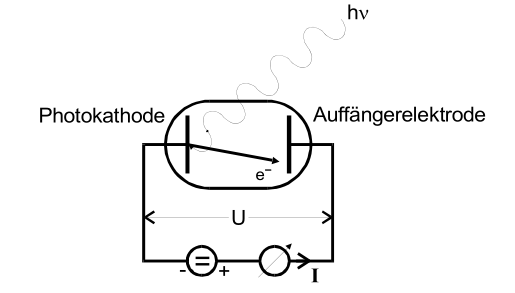
\includegraphics[width = 0.75\textwidth]{data/prinzAnordnung.png}
    \caption{Prinzipielle Anordnung des Versuches zum Photoeffekt \cite{Anleitung500}.}
    \label{fig:prinzAnordn}
\end{figure}

\noindent
Bei dem Versuch wird ein Strom aus den Elektronen gemessen, die aus der mit monochromatischem Licht bestrahlten Photokathode herausgelöst werden. Die aus
diesem Versuch gewonnenen experimentellen Beobachtungen lassen sich in die folgenden drei Punkte zusammenfassen \cite{Anleitung500}.
\begin{itemize}
    \item[a)] Die Zahl der pro Zeiteinheit ausgelösten Elektronen ist proportional zur Lichtintensität.
    \item[b)] Die Energie der Photoelektronen - gemessen über ihre Geschwindigkeit - ist proportional zur Lichtfrequenz und unabhängig von der Lichtintensität.
    \item[c)] Es existiert eine Grenzfrequenz, unterhalb derer der Photoeffekt nicht auftritt.
\end{itemize}
Zwar lassen sich diese drei Phänomene auch mit dem Wellenmodell erklären, allerdings muss angenommen werden, dass die Energie des Lichtes gleichmäßig über die
ausgestrahlte Wellenfläche verteilt ist. Es ist aber festzustellen, dass die Energie quantisiert in Photonen übertragen wird. Daraus lassen sich die folgenden Erkentnisse
ableiten \cite{Anleitung500}.
\begin{enumerate}
    \item Monochromatisches Licht der Frequenz $\nu$ besteht aus Photonen, die sich mit der Lichtgeschwindigkeit $c$ geradlinig bewegen und die alle die Energie $E=h\nu$ 
        besitzen ($h$ entspricht dem Planck'schen Wirkungsquantum).
    \item Ein Photon überträgt seine Energie momentan auf ein Elektron. Diese teilt sich auf in die sogenannte Austrittsarbeit $W_{\text k}$, das heißt, die Energie, 
        die notwendig ist, damit das Elektron die Festkörperoberfläche verlassen kann, und in die kinetische Energie des Elektrons. Diese Energiebilanz beim Photoeffekt 
        hat somit die Gestalt
        \begin{align}
            \label{eqn:energiebilanz}
            h\nu = E_{\text{kin}} + W_{\text k}.
        \end{align}
        Aus der Gleichung \eqref{eqn:energiebilanz} folgt außerdem die Grenzfrequenz unter derer der Photoeffekt nicht mehr auftreten kann. Des weiteren folgt, dass die kinetische
        Energie proportional zur Frequenz des Lichtes ist.
        \item Die Lichtintensität ist proportional zur Zahl der Photonen pro Zeit- und Raumwinkeleinheit. Da ein Photon höchstens ein Elektron aus der Metalloberfläche lösen kann, kann die Beobachtung a) mit der
            3. Erkentniss erklärt werden.
\end{enumerate}

\noindent
Um die Energie der Photoelektronen zu messen, wird die Gegenfeldmethode verwendet. Somit können nur die Elektronen zur Messanode gelangen, deren kinetische Energie
größer ist als die Energie des angelegten Gegenfeldes. Somit folgt, dass der Strom spätestens dann verschwindet, wenn die folgende Relation 
\begin{align}
    e_0 U_{\text G}=\frac 12 m_0v_{\text{max}}^2
    \label{eqn:stromEnergieRelation}
\end{align}
gilt. Dabei ist $v_{\text{max}}$ die Geschwindigkeit der schnellsten Elektronen, $m_0$ die Ruhemasse des Elektrons und $e_0$ die Elementarladung. Nach den beiden
Gleichungen \eqref{eqn:energiebilanz} und \eqref{eqn:stromEnergieRelation} kann demnach die kinetische Energie der schnellsten Elektronen bestimmt werden,
\begin{align}
    h\nu = e_0 U_{\text G} + A_{\text k}.
    \label{eqn:energieElektr}
\end{align}
Da die Elektronen jedoch nicht monoenergetisch sind, sondern vielmehr eine Energieverteilung haben, fällt der Photostrom bei $U=U_{\text G}$ nicht sofort auf null und fällt
stattdessen bereits bei $U<U_{\text G}$ merklich ab. Die Strom-Spannungskurve sieht in etwa so aus, wie in \autoref{fig:photstrom}. Unter bestimmten Voraussetzungen besteht zwischen der Bremsspannung
und dem Photostrom ein parabolischer Zusammenhang
\begin{align}
    I_{\text{Ph}} \sim U^2.
    \label{eqn:wurzelIGesetz}
\end{align}
Dieser Zusammenhang wird auch dazu genutzt die Spannung $U_{\text G}$ zu bestimmen, indem $\sqrt I$ gegen die Spannung $U$ aufgetragen und $U_{\text{G}}$ 
als Schnittpunkt der erhaltenen Geraden mit der U-Achse bestimmt wird.
\begin{figure}[H]
    \centering
    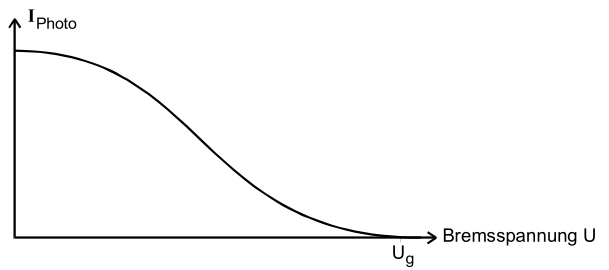
\includegraphics[width = 0.75\textwidth]{data/Photostrom.png}
    \caption{Schematische Darstellung des Stromverlaufes in Abhängigkeit der Bremsspannung \cite{Anleitung500}.}
    \label{fig:photstrom}
\end{figure}